\documentclass[../main.tex]{subfiles}
\graphicspath{{\subfix{../images/}}}
\begin{document}


\section{Surface of revolution}
When we rotate a function about an axis, we can calculate the surface area of the shape formed.

We can work out the formula for this through intuition and combining what we have done with arc lengths and volumes of revolution.

Imagine the surface being made up of a number of circular bands. In other words, similar to the arc length approach, but each small line segment is rotated.

\begin{figure}[h]
    \centering
    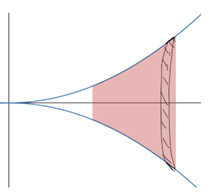
\includegraphics{images/surfacerev1.png}
\end{figure}

\subsection*{Challenge}
Using this approach, try to work out the formula for surface area of a revolution.
\pagebreak
\subsection*{Solution}
\begin{figure}[h]
    \centering
    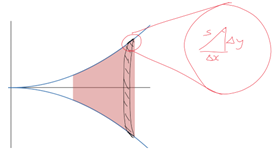
\includegraphics{images/surfacerev2.png}
\end{figure}

As for the arc length approach, the length of each of these line segments could be found by using Pythagoras' Theorem. If the change in $x$ is constant, we can calculate the length of the nth line segment with:

$s_n=\sqrt{(\Delta x)^2+(\Delta y)^2}$

This means we can rewrite the line segment length as $s_n=\sqrt{(\Delta x)^2+(f'(x_n)\times \Delta x)^2}$

Which can be simplified as $s_n=\sqrt{1+(f'(x_n))^2}\Delta x$

Now, if we revolve this line segment around the $x$-axis, it will create a thin circular band, with a length of $2\pi r$ and a width of $\Delta x$. Remember, $r$ is the distance the line segment is away from the $x$-axis, so it is just $f(x)$.

This means the area of the band will be $2\pi \times f(x) \times \sqrt{1+(f'(x))^2}\Delta x$.

And finally, since we summing all of these bands between our lower and upper boundaries, we can set up a definite integral:

\[A=2\pi \int_a^b f(x)\sqrt{1+(f'(x))^2}\, dx\]
\pagebreak
\subsection*{Example}
Find the surface formed by revolving the function $y=2x$ around the $x$-axis, between $x=2$ and $x=4$.

$f(x)=2x$

$f'(x)=2$

$A=2\pi \int_2^4 2x\sqrt{1+2^2}\,dx$

$A=2\pi \int_2^4 2\sqrt{5}x\,dx$

$A=4\sqrt{5}\pi\int_2^4 x\,dx$

$A=4\sqrt{5}\pi\Bigl[\frac{x^2}{2}\Bigr]_2^4$

$A=32\sqrt{5}\pi - 8\sqrt{5}\pi=24\sqrt{5}\pi$
\pagebreak
\subsection*{Questions} 
\label{Surface of revolution}
(Answers - page {\pageref{Surface of revolution answers}})

Evaluate the surface area of the following surfaces of revolution:
\begin{enumerate}[itemsep=0.7cm]
    \item 
    The curve $y=x$ rotated in the $x$-axis between $x=1$ and $x=2$

    \item 
    The curve $y=(x-1)^3$ rotated in the $x$-axis between $x=1$ and $x=3$

    \item 
    The curve $y=\sqrt[3]{x}$ rotated about the \textbf{$y$-axis between $y=2$ and $y=4$}

    \item 
    The curve $y=x^2$ rotated about the \textbf{$y$-axis} between $y=1$ and $y=9$

    \item 
    The curve 
    \begin{equation*}
        \begin{cases}
            x=\sqrt{t}\\
            y=\sqrt{(9-t)}
        \end{cases}
    \end{equation*}
    rotated about the $y$-axis between $t=1$ and $t=5$

    \item 
    (2015 Scholarship exam)

    A solid of revolution is a three-dimensional figure formed by revolving a plane area around a given axis. 

    The surface area of a solid of revolution, which has been revolved 360$^\circ$ around the x-axis, is given by: 

    \[A=2\pi \int_a^b f(x)\sqrt{1+(f'(x))^2}\, dx\]

    Find the area of the surface of revolution obtained when the graph of $f(x)=x^3+\frac{1}{12x}$ from $x=1$ to $x=3$ is rotated 360$^\circ$ about the $x$-axis.

\end{enumerate}


\pagebreak


\end{document}